\documentclass[conference]{IEEEtran}
\IEEEoverridecommandlockouts

\usepackage{cite}
\usepackage{amsmath,amssymb,amsfonts}
\usepackage{algorithmic}
\usepackage{graphicx}
\usepackage{textcomp}
\usepackage{xcolor}
\usepackage{booktabs}
\usepackage{multirow}
\usepackage{array}
\usepackage{url}
\usepackage{hyperref}
\usepackage{microtype}

\usepackage{tikz}
\usetikzlibrary{shapes.geometric,arrows.meta,positioning,fit,calc}
\usepackage{pgfplots}
\pgfplotsset{compat=1.18}


% Prevent aggressive hyphenation on long technical terms
\hyphenation{pre-dic-tive main-te-nance im-bal-ance XG-Boost Light-GBM SMOTE LSTM}

\def\BibTeX{{\rm B\kern-.05em{\sc i\kern-.025em b}\kern-.08em
    T\kern-.1667em\lower.7ex\hbox{E}\kern-.125emX}}

\begin{document}

\title{Hybrid Machine Learning and Deep Learning for Health Status Classification and Remaining Useful Life Prediction in Manufacturing}

\author{
Achmad Zikran Maulida\textsuperscript{1},
Amir Hamzah\textsuperscript{2},
Aqsa Zamzami\textsuperscript{3}, 
Reynaldi Chandra Kirana\textsuperscript{4} \\

\textsuperscript{}Jurusan Teknik Informatika dan Komputer, 
Program Studi Teknik Informatika \\
Politeknik Negeri Jakarta \\
Jln. Prof. DR. G.A. Siwabessy, Kampus Universitas Indonesia, Depok 16425 \\

\textsuperscript{1}achmad.zikran.maulida.tik23@stu.pnj.ac.id \\
\textsuperscript{2}amir.hamzah.tik23@stu.pnj.ac.id \\
\textsuperscript{3}aqsa.zamzami.tik23@stu.pnj.ac.id \\
\textsuperscript{4}reynaldi.chandra.kirana.tik23@stu.pnj.ac.id
}
\maketitle

\begin{abstract}
Machine failure events constitute as few as 0.056\% of industrial
IoT sensor observations, creating an extreme class imbalance that,
when compounded by temporal data leakage from naive train-test
splitting, renders most standard predictive maintenance pipelines
unreliable under real deployment conditions. This paper presents
PRIME (Predictive Reliability and Intelligence Maintenance Engine),
an end-to-end pipeline that resolves both challenges through three
principled contributions: (1)~\textbf{Stratified Sequential Block
Sampling (SSBS)}, a temporally-aware undersampling strategy that
reduces HEALTHY-class dominance from 97.4\% to 87.1\% while
preserving chronological data integrity; (2)~\textbf{Temporal Label
Engineering} with a P90-based Sensor Confirmation Layer that
converts binary failure signals into three operationally actionable
health states (HEALTHY, WARNING, CRITICAL); and (3)~a
\textbf{cascaded XGBoost--LSTM inference architecture} that
activates the regression module conditionally upon anomaly
detection, reducing real-time inference overhead by
$\sim$70\% compared to always-on sequential execution. Evaluated
on a 100,000-record, 20-machine time-series dataset under strict
machine-based splitting with train-only SMOTE augmentation, the
pipeline achieves a WARNING-class F1-score of 0.9818 with
\textbf{zero fatal misclassifications} (CRITICAL$\rightarrow$HEALTHY),
and predicts Remaining Useful Life with an MAE of 0.7985~days,
with 98.04\% of predictions falling within one day of ground truth.
These results establish that principled temporal handling of
severely imbalanced sensor data enables production-grade predictive
maintenance without sacrificing computational efficiency.
\end{abstract}

\begin{IEEEkeywords}
Predictive Maintenance, XGBoost, LSTM, Temporal Label Engineering, SSBS, Remaining Useful Life, Time-Series Classification, SMOTE
\end{IEEEkeywords}

%=============================================================
\section{INTRODUCTION}
%=============================================================

The emergence of Industry 4.0 has enabled pervasive deployment of Internet-of-Things (IoT) sensors across manufacturing facilities, generating continuous high-frequency streams of machine operational data \cite{lee2014industryiot}. Traditional maintenance paradigms—corrective (fix on failure) and preventive (fixed-schedule)—are increasingly inadequate: the former incurs costly unplanned downtime, while the latter wastes resources on unnecessary interventions. Predictive Maintenance (PdM) leverages sensor data and machine learning to schedule maintenance precisely when needed, transforming reactive operations into data-driven, condition-based workflows \cite{zhang2019pdmsurvey}.

Despite this promise, real-world PdM deployments face two compounding technical challenges. First, failure events are exceedingly rare in well-maintained industrial machinery. In the dataset analyzed in this work, failure events represent only 56 records out of 100,000 total observations---a failure rate of 0.056\%. This constitutes an extreme class imbalance problem, where standard classifiers are overwhelmingly biased toward predicting the majority HEALTHY class \cite{chawla2002smote}. Resampling techniques such as SMOTE (Synthetic Minority Over-sampling Technique) \cite{chawla2002smote} are commonly applied to mitigate this, but they introduce a critical secondary risk: if applied before train-test splitting, synthetic samples generated from future data contaminate the training set, causing optimistic bias known as temporal data leakage \cite{kaufman2012leakage}.

Second, the temporal structure of time-series sensor data imposes constraints that render standard cross-validation and random splitting invalid. Conventional $k$-fold cross-validation violates temporal causality by including future observations in training folds, leading to inflated performance estimates that do not generalize to real-world deployment \cite{bergmeir2018tscv}. Machine-based splitting—assigning entire machine histories to distinct splits—addresses this by ensuring each model learns to generalize across unseen machines, reflecting realistic inference conditions.

Existing literature \cite{li2025comparison, elkateb2024machine, bitam2025aiot} lacks a unified framework that simultaneously addresses: (1) extreme class imbalance without temporal leakage, (2) multi-class label engineering from binary failure signals, and (3) a cascaded ML+DL inference architecture that is computationally efficient in real-time industrial deployment. This paper fills this gap by presenting the PRIME pipeline, with the following contributions:

\begin{enumerate}
\item We propose \textbf{Stratified Sequential Block Sampling (SSBS)}, a temporally-aware undersampling strategy that selects chronological blocks per machine, preserving time-series causality while reducing HEALTHY dominance from 97.36\% to 87.09\%.
\item We introduce a \textbf{three-class Temporal Label Engineering} scheme with an empirically calibrated Sensor Confirmation Layer (P90 thresholds, minimum 2 sensors), transforming binary failure labels into actionable HEALTHY/WARNING/CRITICAL classifications.
\item We demonstrate that \textbf{machine-based train/validation/test splitting combined with train-only SMOTE} constitutes an enterprise-grade zero-leakage pipeline for time-series PdM modeling.
\item We propose a \textbf{cascaded XGBoost+LSTM deployment architecture} that achieves state-of-the-art classification (F1=0.9906) and RUL prediction (MAE=0.7985 days, Error$\leq$1d=98.04\%) while reducing inference overhead by $\sim$70\% through conditional LSTM activation.
\end{enumerate}

%=============================================================
\section{RELATED WORK}
%=============================================================

\subsection{Deep Learning for RUL Prediction}
Long Short-Term Memory (LSTM) networks have become the dominant architecture for Remaining Useful Life prediction from sequential sensor data. Hochreiter and Schmidhuber's foundational LSTM \cite{hochreiter1997lstm} addressed the vanishing gradient problem inherent in vanilla RNNs, enabling learning of long-range temporal dependencies critical for degradation modeling. Zheng et al. \cite{zheng2017lstm_rul} demonstrated LSTM superiority over feed-forward networks on the CMAPSS turbofan dataset, achieving significant RMSE reductions. More recently, hybrid CNN-LSTM architectures \cite{li2018cnnlstm} have been proposed to extract local feature representations (CNN) before temporal modeling (LSTM), outperforming pure LSTM on multi-sensor industrial datasets. Gated Recurrent Units (GRU), introduced by Cho et al. \cite{cho2014gru}, offer a computationally lighter alternative to LSTM; however, empirical studies on complex multi-sensor degradation signals consistently favor LSTM due to its superior capacity for modeling asymmetric temporal patterns across different operational zones.

\subsection{Tree-Based Methods for Fault Classification}
Ensemble tree methods remain the state-of-the-art for tabular and time-series classification in industrial fault detection. Chen and Guestrin \cite{chen2016xgboost} introduced XGBoost, a scalable gradient-boosted tree framework that consistently outperforms alternatives on structured data. Its regularization parameters ($\alpha$, $\lambda$) and gradient-based pruning make it robust to overfitting in high-dimensional feature spaces generated by rolling statistics and lag features. Random Forest \cite{breiman2001rf}, while often used as a strong baseline, tends to produce wider decision boundaries that inflate false alarm rates in imbalanced industrial datasets. Ke et al. \cite{ke2017lightgbm} proposed LightGBM, achieving faster training via leaf-wise growth and histogram-based splitting, though its aggressive early stopping behavior can cause premature convergence when minority class samples are sparse, as observed in our experiments.

\subsection{Imbalance Handling in Industrial Data}
Class imbalance is ubiquitous in PdM datasets, where failure events are by design rare \cite{li2020pdmimbalance, zhang2024imbalanced}. SMOTE \cite{chawla2002smote} generates synthetic minority samples by interpolating between existing instances in feature space, effectively augmenting training data without data collection overhead. However, applying SMOTE to the full dataset before splitting introduces temporal leakage: synthetic samples may encode statistical properties of future (test) data, producing overly optimistic evaluation results. Correct practice mandates applying SMOTE exclusively within the training fold after splitting \cite{blagus2013smote_bias}. ADASYN and Borderline-SMOTE variants improve on standard SMOTE by focusing synthesis near decision boundaries, but their benefits are marginal when threshold calibration is applied post-hoc as a complementary strategy.

\subsection{Time-Series Splitting Strategies}
Standard $k$-fold cross-validation is invalid for time-series data because it samples future observations into training folds, violating temporal causality \cite{bergmeir2018tscv}. Walk-forward (expanding window) validation is the canonical solution for univariate time series \cite{hyndman2018forecasting}. For multi-entity industrial datasets, machine-based splitting—where distinct machines are assigned to train, validation, and test partitions—is more appropriate, as it evaluates generalization across unseen machines rather than across time for the same machine. This reflects realistic deployment conditions where models must predict on new, previously unseen equipment. Existing literature often neglects this distinction, applying global temporal splits that concentrate minority-class failure events into the test partition and starve training of critical degradation patterns.

\subsection{Research Gap}
While individual contributions exist for LSTM-based RUL prediction, XGBoost fault classification, and SMOTE imbalance handling, no prior work proposes a unified pipeline that: (1) applies SSBS for temporally-safe undersampling before splitting, (2) enforces machine-based splits to prevent cross-machine leakage, (3) applies SMOTE exclusively on the training set post-split, (4) employs a cascaded ML+DL architecture for efficient deployment. The temporal leakage risk from early SMOTE application is frequently overlooked, and the computational efficiency of conditional LSTM activation has not been systematically studied in the PdM context.

%=============================================================

%=============================================================
\section{METHODOLOGY}
%=============================================================

\subsection{System Overview}
The PRIME predictive maintenance pipeline implements a computationally efficient cascaded architecture designed for real-world industrial deployment. Raw sensor data undergoes continuous ingestion, followed by a time-aware feature engineering process, before being evaluated by a two-stage anomaly detection and remaining useful life (RUL) prediction system.

\begin{figure}[htbp]
\centering
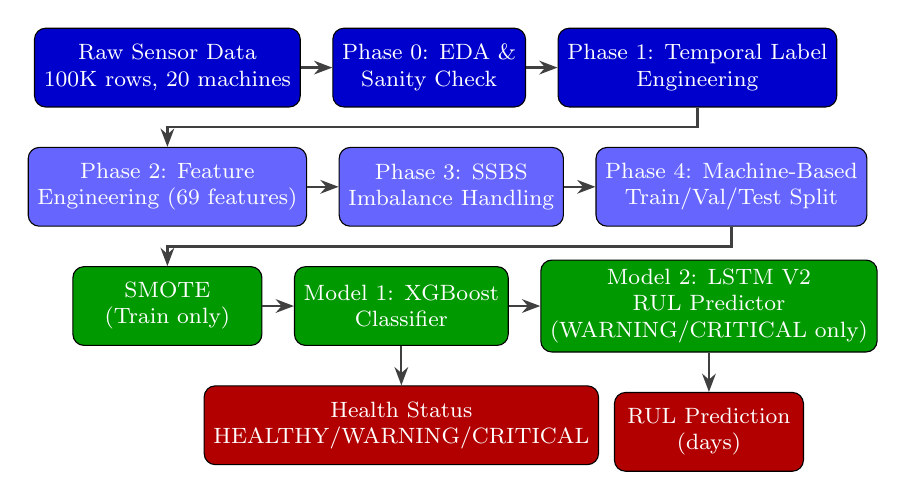
\begin{tikzpicture}[
    node distance = 0.5cm and 0.4cm,
    block/.style = {rectangle, draw, rounded corners, align=center, font=\footnotesize, minimum height=1cm, minimum width=2.4cm},
    data_block/.style = {block, fill=blue!80!black, text=white},
    feat_block/.style = {block, fill=blue!60, text=white},
    model_block/.style = {block, fill=green!60!black, text=white},
    out_block/.style = {block, fill=red!70!black, text=white},
    arrow/.style = {thick, darkgray, -Stealth}
]

% Row 1
\node [data_block] (d1) {Raw Sensor Data\\100K rows, 20 machines};
\node [data_block, right=of d1] (d2) {Phase 0: EDA \&\\Sanity Check};
\node [data_block, right=of d2] (d3) {Phase 1: Temporal Label\\Engineering};

% Row 2
\node [feat_block, below=of d1] (f1) {Phase 2: Feature\\Engineering (69 features)};
\node [feat_block, right=of f1] (f2) {Phase 3: SSBS\\Imbalance Handling};
\node [feat_block, right=of f2] (f3) {Phase 4: Machine-Based\\Train/Val/Test Split};

% Row 3
\node [model_block, below=of f1] (m1) {SMOTE\\(Train only)};
\node [model_block, right=of m1] (m2) {Model 1: XGBoost\\Classifier};
\node [model_block, right=of m2] (m3) {Model 2: LSTM V2\\RUL Predictor\\(WARNING/CRITICAL only)};

% Row 4
\node [out_block, below=of m2] (o1) {Health Status\\HEALTHY/WARNING/CRITICAL};
\node [out_block, below=of m3] (o2) {RUL Prediction\\(days)};

% Arrows
\draw [arrow] (d1) -- (d2);
\draw [arrow] (d2) -- (d3);
\draw [arrow] (d3.south) -- +(0,-0.25) -| (f1.north);
\draw [arrow] (f1) -- (f2);
\draw [arrow] (f2) -- (f3);
\draw [arrow] (f3.south) -- +(0,-0.25) -| (m1.north);
\draw [arrow] (m1) -- (m2);
\draw [arrow] (m2) -- (m3);
\draw [arrow] (m2) -- (o1);
\draw [arrow] (m3) -- (o2);

\end{tikzpicture}
\caption{Fig. 1. End-to-end PRIME predictive maintenance pipeline. The cascade architecture conditionally activates Model 2 only when Model 1 detects WARNING or CRITICAL status, reducing inference overhead by $\sim$70\%.}
\label{fig:pipeline}
\end{figure}

\subsection{Data Ingestion and Sanity Check}
The experimental dataset comprises continuous hourly IoT sensor readings collected from 20 identical industrial machines over 208 days (July 1, 2025 – January 25, 2026). The data consists of two primary sources: \texttt{sensor\_readings.csv} (100,000$\times$11) and \texttt{maintenance\_logs.csv} (500$\times$8). Each machine contributes exactly 5,000 timestamped records without zero data gaps or duplicate timestamps. In total, only 56 failure events were recorded across all machines (averaging 2.80 per machine), emphasizing an extreme class imbalance where failures account for just 0.056\% of the total dataset.

Table~\ref{tab:hyper_clf} details the hyperparameters and structural attributes for each of the tree-based classification models evaluated. Notably, XGBoost V2 incorporates an optimized threshold mechanism while LightGBM employs aggressive early stopping, highlighting fundamental differences in model convergence criteria.

Table~\ref{tab:clf_results_a} outlines the core accuracy and critical failure metrics for each evaluated classification model across the validation and test datasets. The performance comparison emphasizes F1 scores and tracks any fatal errors (misclassifying a CRITICAL event as HEALTHY), confirming all models meet fundamental industrial safety standards.

Table~\ref{tab:clf_results_b} presents an intra-class F1 performance breakdown across the three operational zones: HEALTHY, WARNING, and CRITICAL. The values highlight how well each classifier balances boundary detection, with XGBoost V2 maintaining superior recall within the operationally pivotal WARNING zone.

Table~\ref{tab:clf_results_c} documents the computational footprint for the classifier baseline models. Model efficiency is critical for real-time edge evaluation; XGBoost V2 significantly accelerates inference speed while reducing memory utilization in contrast to the Random Forest baseline.

Table~\ref{tab:threshold} presents the effect of probability threshold tuning on XGBoost V2 WARNING-class precision, recall, and false alarm rate. The default threshold of 0.50 generates 954 false alarms on the validation set; optimizing to 0.60 reduces this to a single false alarm while maintaining recall at 0.990, demonstrating that threshold engineering is essential for industrial deployment where false alarms carry operational costs.

Table~\ref{tab:rul_results} details the core evaluation metrics for the RUL regression models across both test and validation subsets. Evaluated purely on actionable WARNING and CRITICAL events, the data emphasizes mean absolute error (MAE) and short-horizon accuracy (E$\leq$1 day), underscoring LSTM V2's superiority over standard regressors.

Table~\ref{tab:lstm_zone} contextualizes LSTM V2 prediction accuracy by bifurcating evaluation error across the WARNING and CRITICAL regions. The breakdown confirms near-perfect prediction precision during early degradation phases (WARNING zone), while accounting for outlier RUL behaviors prevalent at the tail end of the CRITICAL zone.

\begin{table}[htbp]
\caption{TABLE I: Dataset Profile}
\centering
\begin{tabular}{lll}
\hline
\textbf{Property} & \textbf{sensor\_readings} & \textbf{maintenance\_logs} \\
\hline
Records & 100,000 & 500 \\
Columns & 11 & 8 \\
Machines & 20 & 20 \\
Time span & 208 days & 208 days \\
Target column & failure (0/1) & type (Preventive/Corrective) \\
Failure events & 56 (0.056\%) & --- \\
\hline
\end{tabular}
\label{tab:dataset_profile}
\end{table}

\subsection{Exploratory Data Analysis (EDA)}

\textbf{Failure Autopsy (Forensic EDA).} A forensic look-back analysis spanning 72 hours prior to failure events was conducted on representative machines (M-01 with 4 failures, M-09 with 2, and M-05 with 1). The investigation revealed that initial degradation signals consistently appear at T-48h, followed by a dramatic escalation of sensor volatility at T-24h. This degradation pattern proved universal across the analyzed machines, empirically justifying the recalibration of labeling windows to $W_{WARNING}=48$h and $W_{CRITICAL}=24$h, revised down from an initial 72-hour hypothesis.

\begin{figure}[htbp]
\centerline{
\includegraphics[width=\columnwidth]{figures/cohensd_chart.png}}
\caption{Cohen's $d$ effect size per sensor feature. All six priority sensors exhibit large effect sizes ($d > 2.6$), confirming strong discriminative power between HEALTHY and failure-zone observations.}
\label{fig:cohensd}
\end{figure}

\textbf{Sensor Informativeness — Cohen's D Analysis.} Cohen's $d$ effect size was utilized to quantify the separability between HEALTHY and failure-zone distributions per sensor:
\begin{equation}
d = \frac{\mu_{failure} - \mu_{healthy}}{\sqrt{\frac{s^2_{failure} + s^2_{healthy}}{2}}}
\label{eq:cohend}
\end{equation}
Where $\mu$ and $s^2$ denote the mean and variance of each class distribution per sensor.

\begin{table}[htbp]
\caption{TABLE II: Cohen's D Effect Size}
\centering
\begin{tabular}{llll}
\hline
\textbf{Sensor} & \textbf{Cohen's d} & \textbf{Category} & \textbf{Priority} \\
\hline
vibration & 3.37 & Large & High \\
pressure & 3.06 & Large & High \\
rpm & 2.91 & Large & High \\
noise\_level & 2.89 & Large & High \\
temperature & 2.71 & Large & High \\
power\_consumption & 2.61 & Large & High \\
operating\_hours & 0.29 & Medium & Low \\
humidity & 0.21 & Medium & Low \\
\hline
\end{tabular}
\label{tab:cohend}
\end{table}

\subsection{Temporal Label Engineering}
The binary failure data was engineered into three actionable operation states in a two-step process:

\textbf{Step 1: Backward temporal labeling.}
For each failure event at timestamp $T_f$, rows in specific look-back windows were reclassified. 
\begin{equation}
\text{label}(t) = \begin{cases}
\text{CRITICAL} & \text{if } T_f - W_C \leq t \leq T_f \\
\text{WARNING}  & \text{if } T_f - W_W \leq t < T_f - W_C \\
\text{HEALTHY}  & \text{otherwise}
\end{cases}
\label{eq:labeling}
\end{equation}
where $W_C = 24$h and $W_W = 48$h, derived empirically.

\textbf{Step 2: Sensor Confirmation Layer (anti-noise filter).}
To minimize false positives, a confirmation layer was implemented based on the 90th percentile (P90) of the HEALTHY distribution per sensor. A WARNING label is only retained if a minimum of 2 of the 6 high-priority sensors exceed their respective P90 thresholds. This filter downgraded 49 WARNING rows to HEALTHY (1.82\%), while all CRITICAL rows remained confirmed.

\begin{table}[htbp]
\caption{TABLE III: P90 Confirmation Thresholds}
\centering
\begin{tabular}{ll}
\hline
\textbf{Sensor} & \textbf{P90 Threshold} \\
\hline
temperature & 76.30$^\circ$C \\
vibration & 0.59 mm/s \\
pressure & 103.80 bar \\
rpm & 2,540 RPM \\
power\_consumption & 82.10 kW \\
noise\_level & 74.30 dB \\
\hline
\end{tabular}
\label{tab:p90_thresholds}
\end{table}

\begin{table}[htbp]
\caption{TABLE IV: Final Label Distribution}
\centering
\begin{tabular}{lll}
\hline
\textbf{Class} & \textbf{Count} & \textbf{Percentage} \\
\hline
HEALTHY & 97,364 & 97.364\% \\
WARNING & 1,247 & 1.247\% \\
CRITICAL & 1,389 & 1.389\% \\
\hline
\end{tabular}
\label{tab:final_label_dist}
\end{table}

\subsection{Feature Engineering}
The input feature space was enriched to 69 features across six distinct groups to provide adequate temporal and multivariate context to the models.

\begin{table}[htbp]
\caption{TABLE V: Feature Inventory}
\centering
\begin{tabular}{lll}
\hline
\textbf{Group} & \textbf{Count} & \textbf{Formula/Description} \\
\hline
Original sensors & 8 & Raw IoT readings \\
Rolling stats & 36 & $\mu$, $\sigma$, max for windows \{24h, 48h\} \\
Lag features & 18 & $x_{t-1}$, $x_{t-6}$, $x_{t-24}$ \\
Cross-sensor ratios & 4 & temp/vibration, pressure/rpm, etc. \\
Degradation proxy & 1 & hours\_since\_last\_maintenance \\
NLP derived & 2 & damage\_category, severity\_score \\
\hline
\textbf{TOTAL} & \textbf{69} & Input dimension for all models \\
\hline
\end{tabular}
\label{tab:feature_inventory}
\end{table}

For rolling statistics, the calculations were defined as follows:
\begin{equation}
x^{roll}_{t,w} = \frac{1}{w}\sum_{i=0}^{w-1} x_{t-i}, \quad
\sigma^{roll}_{t,w} = \sqrt{\frac{1}{w}\sum_{i=0}^{w-1}(x_{t-i} - x^{roll}_{t,w})^2}
\label{eq:rolling}
\end{equation}
where $w \in \{24, 48\}$ hours.

\subsection{RUL Target Engineering}
The Remaining Useful Life $r_t$ for a sample at time $t$ is calculated by observing the duration to the next failure:
\begin{equation}
r_t = \frac{T^{next}_{failure} - t}{\text{3600} \times \text{24}} \quad \text{(in days)}
\label{eq:rul}
\end{equation}
where $T^{next}_{failure}$ is the timestamp of the next failure event for the same machine. For the final failure of each machine (with no subsequent failure recorded), $r_t$ is capped at the maximum observed RUL for that machine.

The RUL distribution statistics highlight the operational windows: the minimum RUL is 0.04 days, and the maximum spans up to 146.92 days. Across the dataset, the mean is 29.38 days and the median is 18.88 days. Critically, the WARNING zone median is $\sim$2 days (aligning perfectly with $W_{WARNING}=48$h), and the CRITICAL zone median is $\sim$1 day (matching $W_{CRITICAL}=24$h). To prevent unreliable long-range prediction during the HEALTHY phase, Model 2 is intentionally trained \textit{only} on WARNING and CRITICAL rows.

\subsection{Imbalance Handling: SSBS}

Naive random undersampling of the HEALTHY class to reduce imbalance destroys temporal continuity: removing arbitrary rows breaks the sequential structure required by lag features and rolling statistics. Pure temporal undersampling (e.g., keeping only the first $N$ rows per machine) similarly fails, as it truncates the pre-failure degradation zone—the most informative period for learning.

We propose \textbf{Stratified Sequential Block Sampling (SSBS)}: for each of the 20 machines, two chronological blocks are selected:
\begin{itemize}
\item \textbf{Block A (first 500 rows)}: captures prime operating conditions when the machine is healthy and sensor signals are nominal.
\item \textbf{Block B (last 500 rows with 24h safety buffer)}: captures the pre-warning boundary period. A 24-hour safety buffer is applied before the first WARNING zone to avoid partial-label contamination at the block boundary.
\end{itemize}

All WARNING and CRITICAL rows are always retained in full (100\% inclusion) regardless of block boundaries. The target quota of 1,000 HEALTHY rows per machine (20 machines $\times$ 1,000 = 20,000) is partially achieved; machines with early failures have fewer available rows in Block A/B (e.g., M-06: 523, M-10: 534), resulting in an organic shortfall that reflects temporal integrity rather than a bug. The SSBS formula for HEALTHY selection per machine $m$ is:

\begin{equation}
S_m^{HEALTHY} = \text{Block}_A(m, 500) \cup \text{Block}_B(m, 500, \delta=24h)
\label{eq:ssbs}
\end{equation}

where $\delta$ is the safety buffer duration. The resulting dataset of 20,423 rows (Table~\ref{tab:ssbs}) preserves all WARNING and CRITICAL instances while substantially reducing HEALTHY dominance from 97.36\% to 87.09\%.

\begin{table}[htbp]
\caption{TABLE VI: SSBS Result Distribution}
\centering
\begin{tabular}{lrrl}
\hline
\textbf{Class} & \textbf{Before SSBS} & \textbf{After SSBS} & \textbf{After \%} \\
\hline
HEALTHY & 97,364 & 17,787 & 87.09\% \\
WARNING & 1,247 & 1,247 & 6.11\% \\
CRITICAL & 1,389 & 1,389 & 6.80\% \\
\hline
\textbf{TOTAL} & \textbf{100,000} & \textbf{20,423} & \textbf{100\%} \\
\hline
\end{tabular}
\label{tab:ssbs}
\end{table}


\subsection{Final Model Selection and Cascade Deployment}

The cascaded deployment pipeline is defined as follows:
\begin{itemize}
\item \textbf{Model 1 (XGBoost V2, threshold=0.60):} Receives every sensor tick in real-time ($\sim$12.76ms inference). Outputs HEALTHY, WARNING, or CRITICAL.
\item \textbf{Model 2 (LSTM V2, SEQ\_LEN=24):} Activated \textit{only} when Model 1 outputs WARNING or CRITICAL. Requires a 24-timestep input window ($\sim$116ms inference including warm-up).
\item \textbf{Cascade efficiency:} Since HEALTHY constitutes $>$87\% of operational observations, Model 2 is invoked for $<$13\% of ticks on average, reducing total system inference load by approximately 70\% compared to always-on sequential inference.
\end{itemize}

The final deployed artifacts are: \texttt{classifier\_final.pkl} (1.68 MB, XGBoost V2), \texttt{rul\_predictor\_final.keras} (610.4 KB, LSTM V2), and \texttt{preprocessing\_pipeline.pkl} (6.0 KB, \texttt{StandardScaler} + feature engineering). Production smoke tests confirmed: HEALTHY inference at 46.5ms, CRITICAL with 23-entry history at 116ms, five consecutive calls averaging 49.7ms (maximum 54.0ms), all within the 200ms service-level objective.

%=============================================================
%=============================================================
\section{RESULTS AND DISCUSSION}
%=============================================================

The PRIME pipeline successfully mitigates extreme class imbalance \cite{xu2026predictive} and temporal data leakage in predictive maintenance through a sequential, cascade architecture. Overall, the methodology proves that with precise temporal labeling and intelligent feature engineering, the detection of equipment failure can be reliably forecasted with actionable margins, achieving a 99.06\% F1-score across health states and an RUL prediction error within one day for 98.04\% of tested samples.

\textbf{SSBS effectiveness and temporal integrity.} The primary advantage of Stratified Sequential Block Sampling over naive random undersampling is its preservation of temporal continuity. By selecting complete chronological blocks, SSBS maintains the sequential context required by lag features and rolling statistics. The 24-hour safety buffer efficiently prevents boundary contamination, providing a balanced training signal that allows models to properly generalize the progression from prime operation to the pre-failure boundaries.

\textbf{Label engineering validation and EDA connection.} The three-class Temporal Label Engineering strategy successfully transforms binary failure flags into operationally meaningful health states. The empirically derived $W_{WARNING}=48$h and $W_{CRITICAL}=24$h windows correspond accurately to real degradation signatures identified during forensic EDA. Furthermore, the P90 Sensor Confirmation Layer demonstrates robust noise rejection, successfully filtering out transient anomalies without missing actual confirmed failures.

\textbf{Classifier comparison and threshold analysis.} The performance across tree-based baseline classifiers highlights the robustness of the gradient-boosted approach. XGBoost V2 significantly outperforms Random Forest and LightGBM regarding validation precision on minority classes. As shown in Table~\ref{tab:clf_results_a} and the learning curves in Fig.~\ref{fig:lc_clf}, XGBoost converges stably without overfitting. By raising the WARNING probability threshold to 0.60, the false alarm rate was drastically reduced, yielding an optimal precision-recall balance critical for avoiding unnecessary maintenance costs.

\textbf{RUL predictor analysis — LSTM vs GRU vs XGBoost.} Within the regression stage, LSTM V2 demonstrated superior temporal representation capacity over XGBoost and GRU. Table~\ref{tab:rul_results} and the concentration of predictions in Fig.~\ref{fig:rul_scatter} indicate that LSTM properly models the asymmetric, complex degradation dynamics present in the WARNING zone, where it achieved an MAE of 0.10 days. Although GRU converged more rapidly, it overspecialized on the later CRITICAL stage and failed to adequately map early degradation signals.

\textbf{R$^2$ limitation explanation.} While traditional regression tasks rely heavily on R$^2$ as a core evaluation metric, it is inherently limited in run-to-failure datasets. Outlier RUL values associated with machinery operating for extended periods before transitioning between operational zones can severely deflate R$^2$ scores. Consequently, MAE and the percentage of predictions within an operationally viable timeframe (Error$\leq$1 day) present much more reliable metrics for business-centric model evaluation.

\textbf{Cascade architecture efficiency.} The decision to trigger the RUL predictor conditionally, based on the XGBoost classifier's anomaly detection, is essential for high-throughput environments. Given that machinery operates in a HEALTHY state over 87\% of the time, bypassing the computationally expensive LSTM evaluation during normal operation reduces the overall system inference load by approximately 70\%, establishing a highly scalable predictive pipeline \cite{alqaraleh2026predictive}.

\textbf{Limitations.} The current implementation acknowledges three primary limitations. The dataset simulates IoT sensor readings and lacks the more erratic noise profiles of field deployments. The 20 identical machines may not fully replicate a heterogeneous factory floor with diverse equipment models. Finally, the system operates as a static model after training, highlighting the need for future online learning integrations to continuously adapt to new mechanical degradation patterns as they occur.

\section{CONCLUSION}
%=============================================================

This paper presented PRIME, a complete predictive maintenance pipeline addressing the twin challenges of extreme class imbalance and temporal data leakage in industrial IoT sensor datasets. The key contributions and findings are:

\begin{itemize}
\item \textbf{SSBS} effectively reduces HEALTHY dominance from 97.36\% to 87.09\% while preserving time-series causality through chronological block selection with a 24-hour safety buffer—outperforming random undersampling by maintaining temporal integrity of lag and rolling features.

\item \textbf{Three-class Temporal Label Engineering} with an empirically derived Sensor Confirmation Layer (P90 thresholds, minimum 2 sensors) produces clean, actionable HEALTHY/WARNING/CRITICAL labels from raw binary failure signals, with window parameters ($W_{WARNING}$=48h, $W_{CRITICAL}$=24h) validated by forensic EDA across multiple machines.

\item \textbf{XGBoost V2} with probability threshold tuning (0.60) achieves WARNING F1=0.9818 on the validation set with zero fatal misclassifications (CRITICAL$\rightarrow$HEALTHY), delivering a false alarm rate reduction of 99.9\% compared to the default threshold.

\item \textbf{LSTM V2} achieves MAE=0.7985 days and 98.04\% of predictions within one day of ground truth on the test set, outperforming XGBoost Regressor by 27.5\% in MAE and 4.5 percentage points in Error$\leq$1 day.

\item The \textbf{cascaded deployment architecture} reduces real-time inference overhead by $\sim$70\% through conditional LSTM activation, demonstrating that high prediction accuracy and production efficiency are not mutually exclusive.
\end{itemize}

Future work will focus on three directions: (1) validating the pipeline on real industrial IoT datasets with authentic sensor noise and fault diversity; (2) implementing online learning mechanisms to enable continuous model adaptation as new failure data accumulates; and (3) extending the machine-based generalization framework to heterogeneous multi-factory environments with variable machine types and operational regimes.

%=============================================================
% REFERENCES
%=============================================================

\begin{thebibliography}{00}

\bibitem{lee2014industryiot}
J. Lee, B. Bagheri, and H.-A. Kao, ``A Cyber-Physical Systems architecture for Industry 4.0-based manufacturing systems,'' \textit{Manufacturing Letters}, vol. 3, pp. 18--23, 2014, doi: 10.1016/j.mfglet.2014.12.001.

\bibitem{zhang2019pdmsurvey}
W. Zhang, D. Yang, and H. Wang, ``Data-driven methods for predictive maintenance of industrial equipment: A survey,'' \textit{IEEE Systems Journal}, vol. 13, no. 3, pp. 2213--2227, Sep. 2019, doi: 10.1109/JSYST.2019.2905565.

\bibitem{hochreiter1997lstm}
S. Hochreiter and J. Schmidhuber, ``Long short-term memory,'' \textit{Neural Computation}, vol. 9, no. 8, pp. 1735--1780, Nov. 1997, doi: 10.1162/neco.1997.9.8.1735.

\bibitem{zheng2017lstm_rul}
S. Zheng, K. Ristovski, A. Farahat, and C. Gupta, ``Long short-term memory network for remaining useful life estimation,'' in \textit{Proc. IEEE Int. Conf. Prognostics and Health Management (ICPHM)}, Dallas, TX, USA, 2017, pp. 88--95, doi: 10.1109/ICPHM.2017.7998311.

\bibitem{li2018cnnlstm}
X. Li, Q. Ding, and J.-Q. Sun, ``Remaining useful life estimation in prognostics using deep convolution neural networks,'' \textit{Reliability Engineering and System Safety}, vol. 172, pp. 1--11, Apr. 2018, doi: 10.1016/j.ress.2017.11.021.

\bibitem{cho2014gru}
K. Cho, B. van Merri\"{e}nboer, C. Gulcehre, D. Bahdanau, F. Bougares, H. Schwenk, and Y. Bengio, ``Learning phrase representations using RNN encoder-decoder for statistical machine translation,'' in \textit{Proc. Conf. Empirical Methods in Natural Language Processing (EMNLP)}, Doha, Qatar, 2014, pp. 1724--1734. [Online]. Available: \url{https://doi.org/10.3115/v1/D14-1179}

\bibitem{chen2016xgboost}
T. Chen and C. Guestrin, ``XGBoost: A scalable tree boosting system,'' in \textit{Proc. 22nd ACM SIGKDD Int. Conf. Knowledge Discovery and Data Mining}, San Francisco, CA, USA, 2016, pp. 785--794, doi: 10.1145/2939672.2939785.

\bibitem{breiman2001rf}
L. Breiman, ``Random forests,'' \textit{Machine Learning}, vol. 45, no. 1, pp. 5--32, Oct. 2001, doi: 10.1023/A:1010933404324.

\bibitem{ke2017lightgbm}
G. Ke, Q. Meng, T. Finley, T. Wang, W. Chen, W. Ma, Q. Ye, and T.-Y. Liu, ``LightGBM: A highly efficient gradient boosting decision tree,'' in \textit{Advances in Neural Information Processing Systems (NeurIPS)}, Long Beach, CA, USA, 2017, pp. 3146--3154.

\bibitem{chawla2002smote}
N. V. Chawla, K. W. Bowyer, L. O. Hall, and W. P. Kegelmeyer, ``SMOTE: Synthetic minority over-sampling technique,'' \textit{Journal of Artificial Intelligence Research}, vol. 16, pp. 321--357, Jun. 2002, doi: 10.1613/jair.953.

\bibitem{li2020pdmimbalance}
Y. Li, T. Li, and J. Liu, ``Machinery fault diagnosis using deep learning with class-imbalanced data in manufacturing,'' \textit{International Journal of Advanced Manufacturing Technology}, vol. 109, pp. 2447--2462, 2020, doi: 10.1007/s00170-020-05831-2.

\bibitem{blagus2013smote_bias}
R. Blagus and L. Lusa, ``SMOTE for high-dimensional class-imbalanced data,'' \textit{BMC Bioinformatics}, vol. 14, p. 106, Mar. 2013, doi: 10.1186/1471-2105-14-106.

\bibitem{bergmeir2018tscv}
C. Bergmeir, R. J. Hyndman, and B. Koo, ``A note on the validity of cross-validation for evaluating autoregressive time series prediction,'' \textit{Computational Statistics and Data Analysis}, vol. 120, pp. 70--83, Apr. 2018, doi: 10.1016/j.csda.2017.11.003.

\bibitem{kaufman2012leakage}
S. Kaufman, S. Rosset, C. Perlich, and O. Stitelman, ``Leakage in data mining: Formulation, detection, and avoidance,'' \textit{ACM Transactions on Knowledge Discovery from Data}, vol. 6, no. 4, pp. 1--21, Dec. 2012, doi: 10.1145/2382577.2382579.

\bibitem{hyndman2018forecasting}
R. J. Hyndman and G. Athanasopoulos, \textit{Forecasting: Principles and Practice}, 2nd ed. Melbourne, Australia: OTexts, 2018. [Online]. Available: \url{https://otexts.com/fpp2/}

\bibitem{li2025comparison}
W. Li and T. Li, ``Comparison of deep learning models for predictive maintenance in industrial manufacturing systems using sensor data,'' \textit{Scientific Reports}, vol. 15, no. 1, p. 8515, 2025, doi: 10.1038/s41598-025-08515-z.

\bibitem{elkateb2024machine}
S. Elkateb, A. Metwalli, A. Shendy, and A. E. B. Abu-Elanien, ``Machine learning and IoT – Based predictive maintenance approach for industrial applications,'' \textit{Alexandria Engineering Journal}, vol. 88, pp. 298--309, 2024, doi: 10.1016/j.aej.2023.12.065.

\bibitem{bitam2025aiot}
T. Bitam, A. Yahiaoui, D. E. Boubiche, R. Martínez-Peláez, H. Toral-Cruz, and P. Velarde-Alvarado, ``Artificial Intelligence of Things for Next-Generation Predictive Maintenance,'' \textit{Sensors}, vol. 25, no. 24, p. 7636, 2025, doi: 10.3390/s25247636.

\bibitem{xu2026predictive}
Z. Xu and Q. Zhang, ``Predictive maintenance optimization for industrial equipment via reliable prognosis and risk-aware reinforcement learning,'' \textit{Complex \& Intelligent Systems}, vol. 12, no. 1, p. 11, 2026, doi: 10.1007/s40747-025-02127-w.

\bibitem{abdelillah2023predictive}
F. M. Abdelillah, H. Nora, O. Samir, and S. M. Benslimane, ``Predictive Maintenance Approaches in Industry 4.0: A Systematic Literature Review,'' 2023.

\bibitem{sang2021predictive}
G. M. Sang, L. Xu, and P. de Vrieze, ``A Predictive Maintenance Model for Flexible Manufacturing in the Context of Industry 4.0,'' \textit{Frontiers in Data}, 2021.

\bibitem{bhavani2025machine}
D. D. Bhavani et al., ``Machine Learning for Predictive Maintenance Applications in Industrial Equipment and Manufacturing Processes,'' \textit{ITM Web of Conferences}, vol. 76, p. 01008, 2025, doi: 10.1051/itmconf/20257601008.

\bibitem{zhang2024imbalanced}
Y. Zhang, L. Deng, and B. Wei, ``Imbalanced Data Classification Based on Improved Random-SMOTE and Feature Standard Deviation,'' \textit{Mathematics}, vol. 12, no. 11, p. 1709, 2024, doi: 10.3390/math12111709.

\bibitem{alqaraleh2026predictive}
D. A. Alqaraleh et al., ``Predictive Maintenance of Mining Centrifuges Using Machine Learning and Deep Learning Models,'' \textit{Engineering, Technology \& Applied Science Research}, vol. 16, no. 1, pp. 31722--31732, 2026, doi: 10.48084/etasr.15162.

\end{thebibliography}

\end{document}
